%%%%%%%%%%%%%%%%%%%%%%%%%%%%%%%%%%%%%%%%%
% Beamer Presentation
% LaTeX Template
% Version 1.0 (10/11/12)
%
% This template has been downloaded from:
% http://www.LaTeXTemplates.com
%
% License:
% CC BY-NC-SA 3.0 (http://creativecommons.org/licenses/by-nc-sa/3.0/)
%
%%%%%%%%%%%%%%%%%%%%%%%%%%%%%%%%%%%%%%%%%

%----------------------------------------------------------------------------------------
%	PACKAGES AND THEMES
%----------------------------------------------------------------------------------------

\documentclass{beamer}

\mode<presentation> {

% The Beamer class comes with a number of default slide themes
% which change the colors and layouts of slides. Below this is a list
% of all the themes, uncomment each in turn to see what they look like.

%\usetheme{default}
%\usetheme{AnnArbor}
%\usetheme{Antibes}
%\usetheme{Bergen}
%\usetheme{Berkeley}
%\usetheme{Berlin}
%\usetheme{Boadilla}
%\usetheme{CambridgeUS}
%\usetheme{Copenhagen}
%\usetheme{Darmstadt}
%\usetheme{Dresden}
%\usetheme{Frankfurt}
%\usetheme{Goettingen}
%\usetheme{Hannover}
%\usetheme{Ilmenau}
%\usetheme{JuanLesPins}
%\usetheme{Luebeck}
%\usetheme{Madrid}
%\usetheme{Malmoe}
%\usetheme{Marburg}
%\usetheme{Montpellier}
%\usetheme{PaloAlto}
%\usetheme{Pittsburgh}
%\usetheme{Rochester}
%\usetheme{Singapore}
%\usetheme{Szeged}
\usetheme{Warsaw}

% As well as themes, the Beamer class has a number of color themes
% for any slide theme. Uncomment each of these in turn to see how it
% changes the colors of your current slide theme.

%\usecolortheme{albatross}
%\usecolortheme{beaver}
%\usecolortheme{beetle}
%\usecolortheme{crane}
%\usecolortheme{dolphin}
%\usecolortheme{dove}
%\usecolortheme{fly}
%\usecolortheme{lily}
%\usecolortheme{orchid}
%\usecolortheme{rose}
%\usecolortheme{seagull}
\usecolortheme{seahorse}
%\usecolortheme{whale}
%\usecolortheme{wolverine}

%\setbeamertemplate{footline} % To remove the footer line in all slides uncomment this line
%\setbeamertemplate{footline}[page number] % To replace the footer line in all slides with a simple slide count uncomment this line

%\setbeamertemplate{navigation symbols}{} % To remove the navigation symbols from the bottom of all slides uncomment this line
}

\usepackage{graphicx} % Allows including images
\usepackage{booktabs} % Allows the use of \toprule, \midrule and \bottomrule in tables

\usepackage{multicol}
\usepackage[portuguese]{babel}
\usepackage[utf8]{inputenc}
%----------------------------------------------------------------------------------------
%	TITLE PAGE
%----------------------------------------------------------------------------------------

\title[Projeto Pindí]{Projeto Pindí} % The short title appears at the bottom of every slide, the full title is only on the title page

\author{João Machado, José Armando Neto, José Pedro Neto, Lucas Moura, 
Marcos Ramos, Maria Santos, Matheus Pimenta, Pablo Urbizagastegui1, Rodrigo Melo, Thaynara Santana, Tuane Fonseca, Vanessa Ribeiro} % Your name
\institute[UnB] % Your institution as it will appear on the bottom of every slide, may be shorthand to save space
{
Universidade de Brasília \\ % Your institution for the title page
\medskip
%\textit{1jpsneto@gmail.com} % Your email address
}
\date{\today} % Date, can be changed to a custom date

\begin{document}

\begin{frame}
\titlepage % Print the title page as the first slide
\end{frame}

\begin{frame}
\frametitle{Agenda} % Table of contents slide, comment this block out to remove it
\tiny \begin{multicols}{2}
  \tableofcontents
\end{multicols}% Throughout your presentation, if you choose to use \section{} and \subsection{} commands, these will automatically be printed on this slide as an overview of your presentation
\end{frame}

%----------------------------------------------------------------------------------------
%	PRESENTATION SLIDES
%----------------------------------------------------------------------------------------

%------------------------------------------------
%------------------------------------------------

\section{Introdução}
\subsection{Resumo da Proposta}
\begin{frame}
  \begin{itemize}
      \item Gestão do tempo;
      \item Atividades de limpeza;
      \item Pindí: sistema autônomo de limpeza.
  \end{itemize}
\end{frame}

\section{Eletrônica}
\subsection{Motores de Passo}
\begin{frame}
  Motores de Passo:
        \begin{itemize}
            \item Sustituição dos Motores DC devido imprecisão;
            \item Mais torque;
            \item Melhor controle de velocidade;
            \item Rotação precisa com malha aberta;
            \item Não há necessidade de alta velocidade.
        \end{itemize}
    \begin{figure}
    \centering
    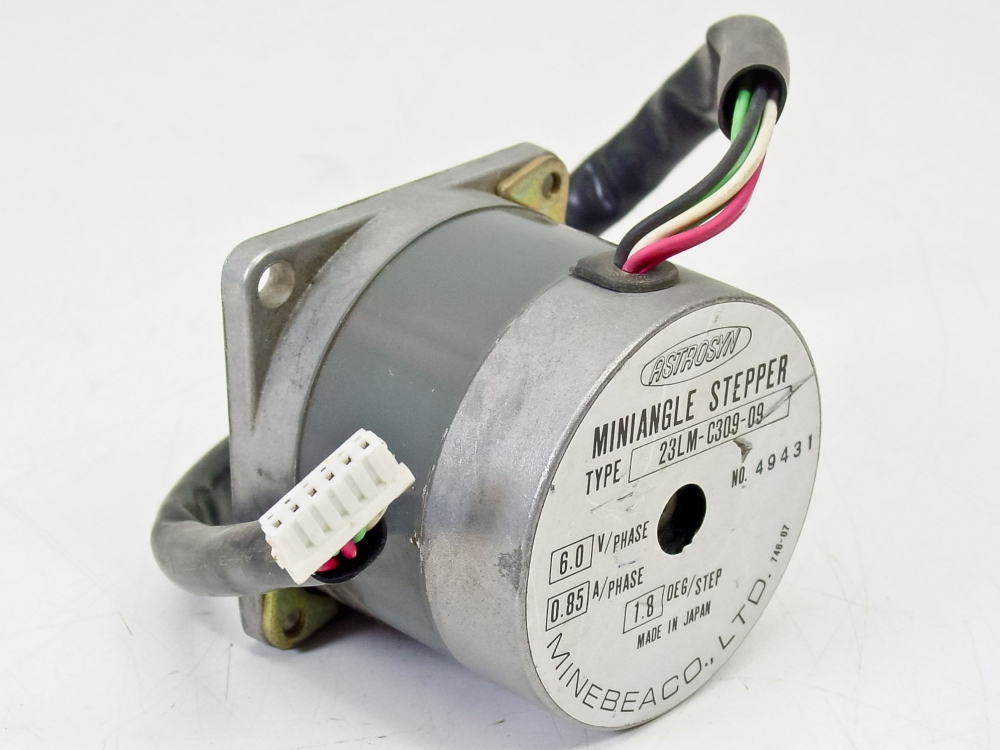
\includegraphics[width=0.4\linewidth]{eletronica_1}
  \end{figure}
\end{frame}

\subsection{Máquina de Estados}
\begin{frame}
  Máquina de Estados:
        \begin{itemize}
            \item Abordagem do controle de movimentação por Máquina de estados.
        \end{itemize}
    \begin{figure}
    \centering
    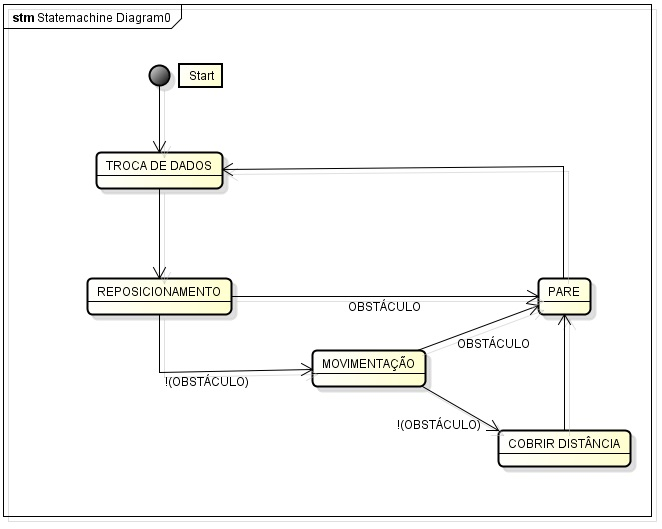
\includegraphics[width=0.63\linewidth]{eletronica_2}
  \end{figure}
\end{frame}

\subsection{Modelo de Circuito Utilizado}
\begin{frame}
  Modelo de Circuito Utilizado
    \begin{figure}
    \centering
    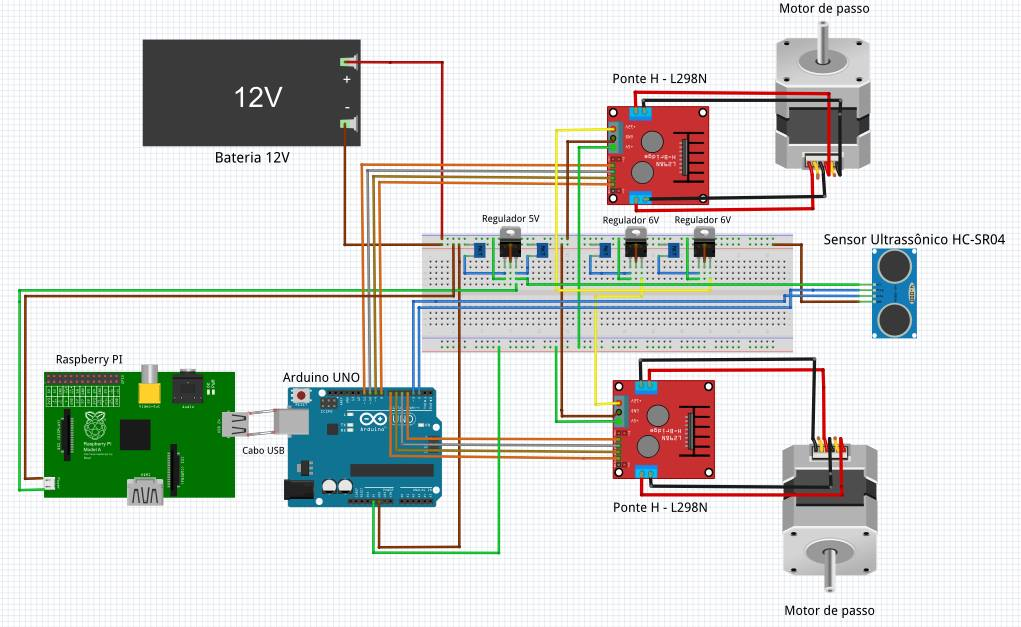
\includegraphics[width=0.9\linewidth]{eletronica_3}
  \end{figure}
\end{frame}


%------------------------------------------------
\section{Software}
\subsection{Software}
\begin{frame}
  \centering
  Focos de atuação em software:
    \begin{itemize}
    \centering
        \item Movimentação: determinação de como o robô se movimentará;
        \centering
        \item Comunicação: determinação de como o centro de controle se comunicará com os periféricos;
    \end{itemize}
\end{frame}

\subsection{Movimentação}
\begin{frame}
  Movimentação:
    \begin{itemize}
        \item Criar mapa usando matrix 2X2;
        \item Estrutura de grafo para garantir movimentação;
        \item Explorar vizinhos usando busca em largura;
        \item Determinar caminhos usando A*.
    \end{itemize}
\end{frame}

\subsection{Exemplo Movimentação}
\begin{frame}
  Exemplo Movimentação
    \begin{figure}
    \centering
    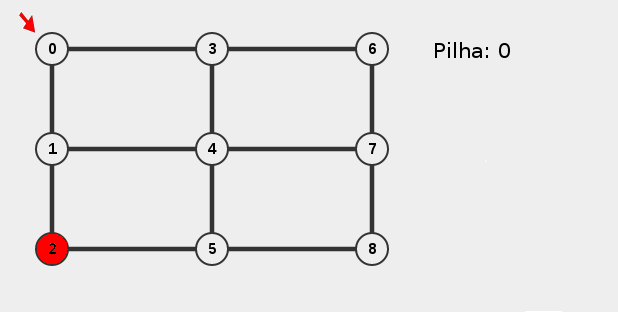
\includegraphics[width=0.9\linewidth]{software_1}
  \end{figure}
\end{frame}

%------------------------------------------------
\subsection{Comunicação}
\begin{frame}
  \centering
  Comunicar mestre e servo através de comunicação serial. Para tal deve-se:
    \begin{itemize}
        \item Definir regras de comunicação entre mestre e escravo;
        \item Garantir a ausência de espera eterna;
        \item Garantir a entrega da mensagem.
    \end{itemize}
    \begin{figure}
    \centering
    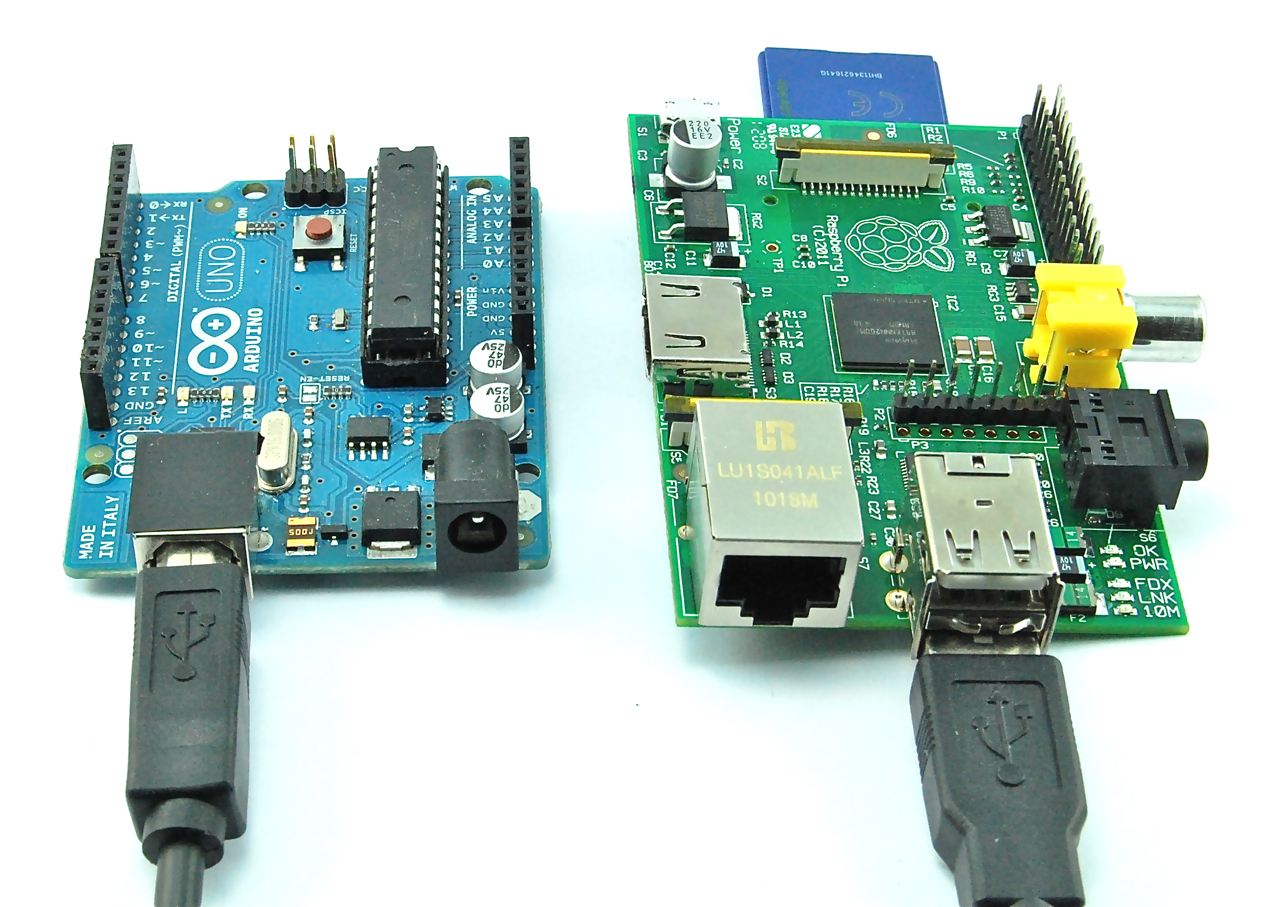
\includegraphics[width=0.4\linewidth]{arduinopi}
  \end{figure}
\end{frame}

\subsection{Visão Geral da Comunicação}
\begin{frame}
  Visão Geral da Comunicação:
    \begin{figure}
    \centering
    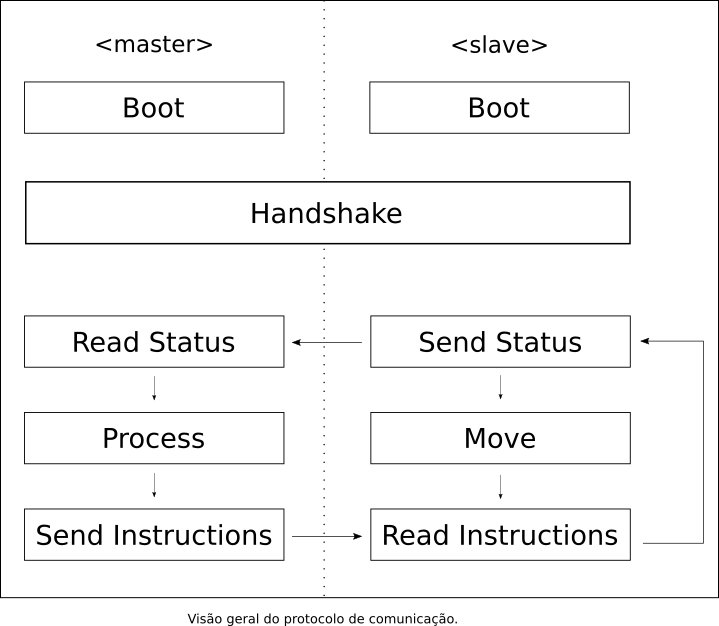
\includegraphics[width=0.6\linewidth]{visao-geral}
  \end{figure}
\end{frame}

\subsection{Handshake}
\begin{frame}
  \centering
  Handshake
    \begin{figure}
    \centering
    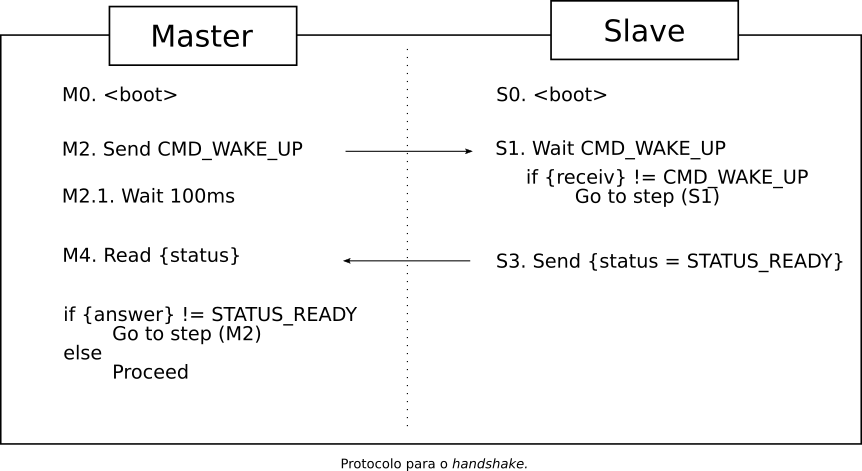
\includegraphics[width=0.5\linewidth]{handshake}
  \end{figure}
   \begin{figure}
    \centering
    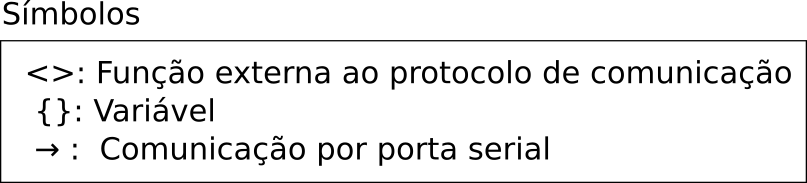
\includegraphics[width=0.5\linewidth]{legenda}
  \end{figure}
\end{frame}

\subsection{Empacotamento dos dados - pacotes TLV}
\begin{frame}
  \centering
  Empacotamento dos dados - pacotes TLV:
    \begin{itemize}
        \item Cabeçalho fixo;
        \item Payload variável;
        \item Possibilita a inserção de novos tipos de dados sem alterar o código de leitura/escrita.
    \end{itemize}
    \begin{figure}
    \centering
    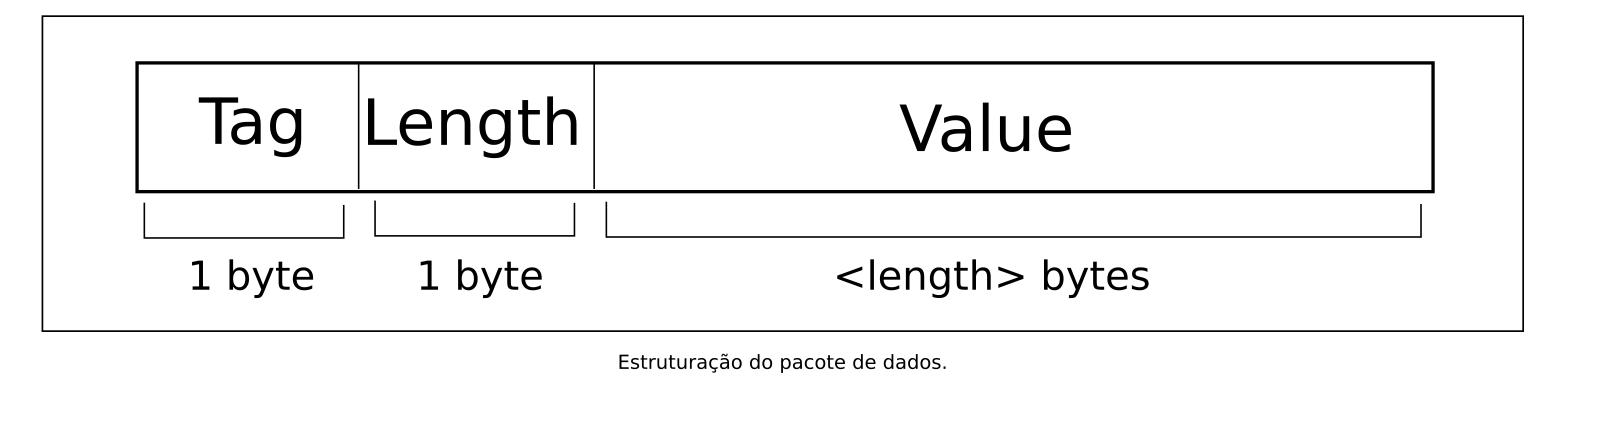
\includegraphics[width=0.9\linewidth]{tlv}
  \end{figure}
\end{frame}

\subsection{Empacotamento dos dados - pacotes TLV}
\begin{frame}
  \centering
  Empacotamento dos dados - pacotes TLV:
    \begin{figure}
    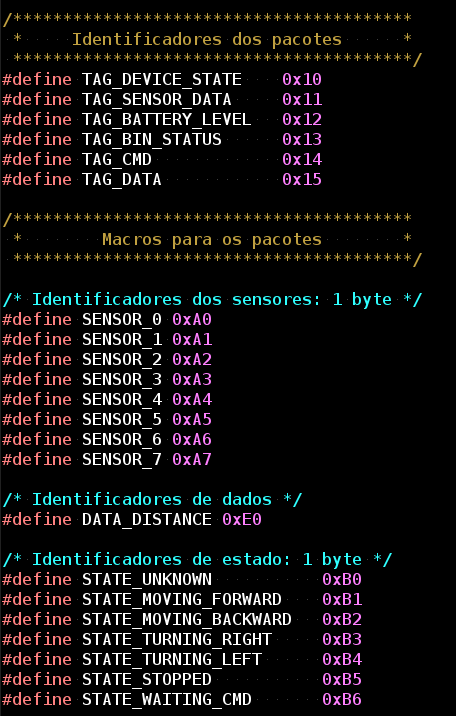
\includegraphics[width=0.35\linewidth]{def_a}
    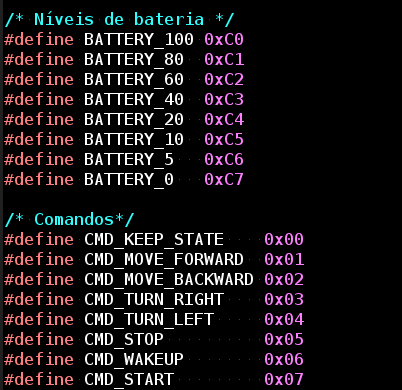
\includegraphics[width=0.35\linewidth]{def_b}
  \end{figure}
\end{frame}

%------------------------------------------------
\section{Automotiva}
\subsection{Projeto da Estrutura - Material e Arranjo}
\begin{frame}
  Escolha do material:
    \begin{itemize}
        \item Peso suportado;
        \item Propriedades físicas.
    \end{itemize}
    Determinação do arranjo:
    \begin{itemize}
        \item Equipe à equipe;
        \item Definidos dimensões e requisitos de localização;
        \item Cálculo de CG por elemento;
        \item Distribuição de peso.
    \end{itemize}
\end{frame}

\subsection{Projeto da Estrutura - Peças e Estruturas}
\begin{frame}
Definição das peças:
    \begin{itemize}
        \item Modelo em CATIA;
        \item Definição exata da geometria;
        \item Testes de resistência.
    \end{itemize}
    Confecção da estrutura:
    \begin{itemize}
        \item Corte da madeira;
        \item Inserção dos suportes;
        \item Acoplamento dos elementos físicos.
    \end{itemize}
\end{frame}

\subsection{Estrutura}
\begin{frame}
    \centering
    Estrutura    
    \begin{figure}
    \centering
    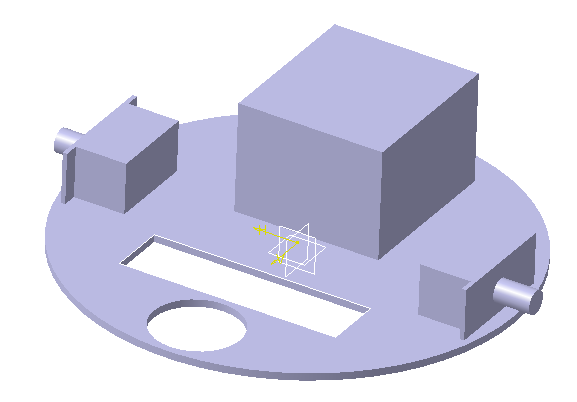
\includegraphics[width=0.8\linewidth]{automotiva_1}
  \end{figure}
\end{frame}
%------------------------------------------------
\section{Energia}
\subsection{Teste em Bateria de Lítio}
\begin{frame}
  Teste em Bateria de Lítio:
        \begin{figure}
          \centering
          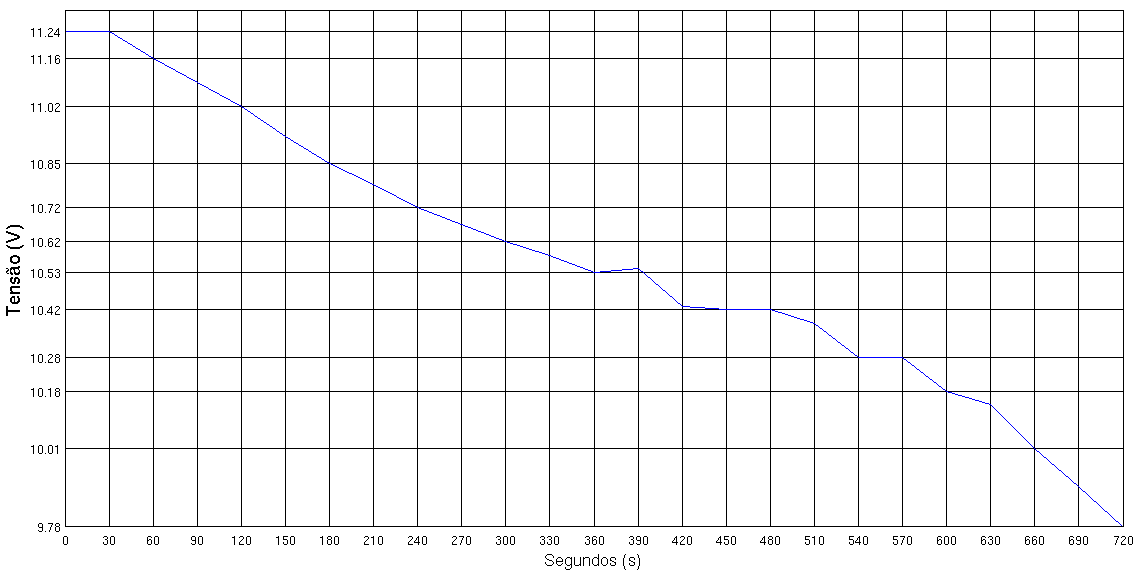
\includegraphics[width=1\linewidth]{energia_1}
          %\caption{Gráfico de Teste em Bateria de Lítio}
        \end{figure}
\end{frame}

\subsection{Teste em Bateria de Chumbo}
\begin{frame}
  Teste em Bateria de Chumbo:
        \begin{figure}
          \centering
          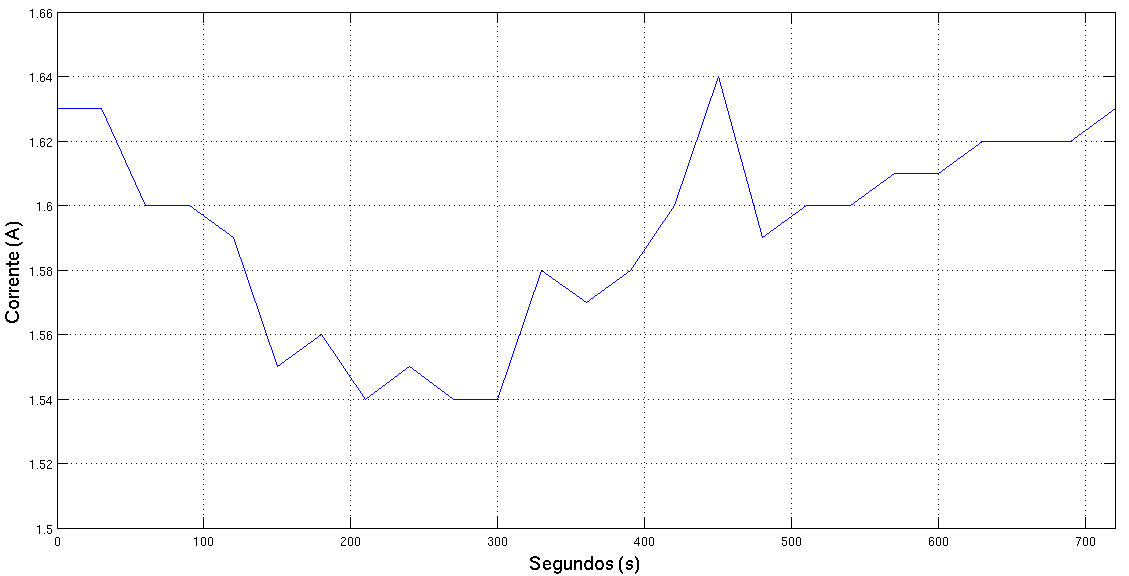
\includegraphics[width=1\linewidth]{energia_2}
          %\caption{Gráfico de Teste em Bateria de Lítio}
        \end{figure}
\end{frame}

%------------------------------------------------
\section{Limpeza}
\subsection{Sistema de Varrição}
\begin{frame}
  Sistema de Varrição:
    \begin{itemize}
        \item Primeiro estágio - protótipo de teste;
        \begin{figure}
          \centering
          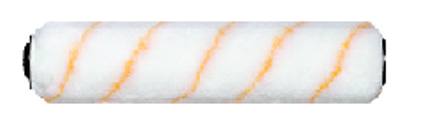
\includegraphics[width=0.8\linewidth]{limpeza_1}
          \caption{Protótipo com motor DC: 9V/0.1A - 300 RPM}
        \end{figure}
        \item Segundo estágio:
        \begin{itemize}
          \item Elaboração do sistema com encaixes;
          \item Desenho CAD;
          \item Simulação no software Ansys CFX.
        \end{itemize}
    \end{itemize}
\end{frame}

\subsection{Sistema de Sucção}
\begin{frame}
  Sistema de Varrição:
    \begin{itemize}
        \item Primeiro estágio:;
        \begin{itemize}
          \item Motor DC 12V/2A - 3600 RPM;
          \item Garrafas PET 500 ml;
          \item Hélice de ventoinha de dissipador de calor.
        \end{itemize}
        \item Segundo estágio:
        \begin{itemize}
          \item Idealização de um novo sistema;
          \item Desenho CAD;
          \item Simulação do fluxo de ar no software Ansys CFX;
          \item Teoria.
        \end{itemize}
    \end{itemize}
\end{frame}

%------------------------------------------------
\section{Fim}
\subsection{Fim}
\begin{frame}
\Huge{\centerline{Obrigado!}}
\end{frame}

%----------------------------------------------------------------------------------------

\end{document} 
